\section{Representations of the Virasoro Algebra}

In the previous sections, we established the deep structural link between local primary operators on the complex plane and highest-weight states defined in the framework of radial quantization. \uline{The local conformal symmetry of a two-dimensional conformal field theory is completely encoded in the \textbf{Virasoro algebra}}:
\[
    [L_m, L_n] = (m - n)L_{m+n} + \frac{c}{12}(m^3 - m)\delta_{m+n,0},
\]
accompanied by an independent copy for the anti-holomorphic sector governing the \(\bar{z}\)-dependence.

The ultimate goal of studying the representation theory of this infinite-dimensional algebra is to classify and organize the entire operator content of the theory. Physically, the full state space (or Hilbert space) \(\mathcal{H}_c\) of a unitary 2D CFT decomposes into a \textit{direct sum of irreducible representations of the holomorphic and anti-holomorphic Virasoro algebras}, labeled by the \textbf{central charge} \(c\) and the \textbf{conformal weights} \((h, \bar{h})\):
\[
    \mathcal{H}_c = \bigoplus_{h, \bar{h}} N_{h, \bar{h}} \mathrm{Vir}_c(h) \otimes \bar{\mathrm{Vir}}_{c}(\bar{h}),
\]
where the non-negative integers \(N_{h, \bar{h}}\) act as multiplicity coefficients, dictating how many times a specific conformal family \((\mathrm{Vir}_c(h) \otimes \bar{\mathrm{Vir}}_{c}(\bar{h}))\) appears in the physical spectrum.

\subsection{Structure of Verma Modules and Level Decomposition}

To systematically construct these representations, we focus heavily on the holomorphic sector, as the anti-holomorphic structure is entirely analogous. Let \(\ket{h}\) be a highest-weight state in the holomorphic sector. By definition, it satisfies the eigenvalue equation for the zero-mode generator and is annihilated by all positive Virasoro modes:
\[
    L_0\ket{h} = h\ket{h}, \quad L_n\ket{h} = 0 \quad (n > 0).
\]
Similarly, we have an anti-holomorphic highest-weight state \(\ket{\bar{h}}\) satisfying:
\[
    \bar{L}_0\ket{\bar{h}} = \bar{h}\ket{\bar{h}}, \quad \bar{L}_n\ket{\bar{h}} = 0 \quad (n > 0).
\]

Starting from this fundamental ground state \(\ket{h}\), we can systematically generate new states by acting with arbitrary combinations of the negative Virasoro modes \(L_{-n_i}\) (with \(n_i > 0\)), which act algebraically as creation operators. A generic state in the representation built on \(\ket{h}\) is a linear combination of monomials of the form:
\[
    L_{-n_1} L_{-n_2} \cdots L_{-n_k} \ket{h}, \quad n_i > 0.
\]
The algebraic structure of the Virasoro algebra naturally induces a \textit{grading} on this representation, organized by the eigenvalue of the dilatation generator \(L_0\). Using the fundamental commutation relation:
\[
    [L_0, L_{-n}] = n L_{-n},
\]
we can evaluate how \(L_0\) acts on a generic state by systematically commuting it to the right until it hits the highest-weight state. For a single mode, we have \(L_0 L_{-n}\ket{h} = (L_{-n}L_0 + nL_{-n})\ket{h} = (h+n)L_{-n}\ket{h}\). By induction, for an arbitrary string of negative modes, one finds that the state:
\[
    L_{-n_1} L_{-n_2} \cdots L_{-n_k} \ket{h}
\]
is a simultaneous eigenstate of \(L_0\) with eigenvalue:
\[
    L_0 \left( L_{-n_1} \cdots L_{-n_k} \ket{h} \right) = (h + N)\ket{h}, \quad \text{where } N = n_1 + n_2 + \dots + n_k.
\]
The non-negative integer \(N\) is defined as the \textbf{level} of the descendant state. Consequently, the entire representation space decomposes into an infinite direct sum of finite-dimensional vector subspaces of fixed level:
\[
    \mathcal{V}_{c,h} = \bigoplus_{N=0}^{\infty} \mathcal{V}_{c,h}^{(N)},
\]
where \(\mathcal{V}_{c,h}\) denotes the complete \textbf{Verma module} characterized by central charge \(c\) and highest weight \(h\), and \(\mathcal{V}_{c,h}^{(N)}\) is the specific subspace containing all descendant states at level \(N\).

As we remarked previously, the states generated by freely applying negative modes are not linearly independent due to the inner commutation relations of the Virasoro algebra itself. For instance, at level 3, the relation \([L_{-1}, L_{-2}] = -L_{-3}\) implies that \(L_{-1}L_{-2}\ket{h}\) can be rewritten in terms of \(L_{-2}L_{-1}\ket{h}\) and \(L_{-3}\ket{h}\). \uline{To systematically avoid overcounting and establish a rigorous basis for each subspace} \(\mathcal{V}_{c,h}^{(N)}\), \uline{we must impose a strict decreasing ordering convention on the indices of the modes:}
\[
    n_1 \ge n_2 \ge \dots \ge n_k \ge 1.
\]

Thus, the Verma module \(\mathcal{V}_{c,h}\) is formally defined as the vector space spanned by all such ordered monomials acting on the highest-weight state:
\[
    \mathcal{V}_{c,h} = \mathrm{span} \left\{ L_{-n_1} L_{-n_2} \cdots L_{-n_k} \ket{h} \; \Big| \; n_1 \ge n_2 \ge \dots \ge n_k \ge 1 \right\}.
\]

Let us explicitly list the basis states for the first few low-lying levels \(N\) to clearly visualize this hierarchy:
\begin{itemize}
    \item \textbf{Level 0:} Contains only the highest-weight state itself, which acts as the primary state:
          \[
              \ket{h}
          \]
    \item \textbf{Level 1:} Generated by the single negative mode \(L_{-1}\):
          \[
              L_{-1}\ket{h}
          \]
    \item \textbf{Level 2:} Formed by two ordered combinations, corresponding to:
          \[
              L_{-2}\ket{h}, \quad L_{-1}^2\ket{h}
          \]
    \item \textbf{Level 3:} Formed by three independent ordered combinations:
          \[
              L_{-3}\ket{h}, \quad L_{-2}L_{-1}\ket{h}, \quad L_{-1}^3\ket{h}
          \]
    \item \textbf{Level 4:} Formed by five independent ordered combinations:
          \[
              L_{-4}\ket{h}, \quad L_{-3}L_{-1}\ket{h}, \quad L_{-2}^2\ket{h}, \quad L_{-2}L_{-1}^2\ket{h}, \quad L_{-1}^4\ket{h}
          \]
\end{itemize}

By inspecting this explicit construction, it becomes evident that the dimension of the subspace \(\mathcal{V}_{c,h}^{(N)}\) at level \(N\) corresponds exactly to the number of ways the integer \(N\) can be expressed as a sum of positive integers, without regard to order. This is precisely the definition of \(p(N)\), the \textbf{number of integer partitions} of \(N\).

The problem of computing \(p(N)\) for any level \(N\) was solved elegantly by Euler through the introduction of a generating function in a formal complex variable \(q\). By defining the generating function \(\varphi(q)\), we can express the dimensions of all level subspaces simultaneously via a formal Taylor expansion:
\[
    \varphi(q) = \prod_{k=1}^{\infty} \frac{1}{1 - q^k} = \sum_{N=0}^{\infty} p(N)q^N.
\]

Each term \(1/(1-q^k)\) in the infinite product can be expanded as a geometric series \(\sum_{m=0}^{\infty} q^{mks}\), where \(m\) physically represents the number of times the Virasoro mode \(L_{-k}\) is applied to the state. When multiplying out the entire product, the coefficient of \(q^N\) automatically counts every possible ordered combination of modes whose total indices sum up to \(N\). Miraculously, all coefficients in this Taylor expansion are positive integers, matching the exact number of linearly independent descendant states at each level in a generic Verma module.

\section{Unitarity Constraints}

In any physical quantum theory, the fundamental requirement of unitarity guarantees the conservation of probability. Mathematically, this dictates that the Hilbert space of states must possess a positive-definite inner product: the norm of any physical state must be strictly non-negative, and there can be no ``ghost'' states (states with negative norm). In the context of a two-dimensional conformal field theory, requiring the absence of negative-norm states in the representation spaces (the Verma modules) imposes severe and profound constraints on the allowed values of the central charge \(c\) and the conformal dimensions \(h\).

\subsection{Hermitian Conjugation and Inner Product}

To systematically evaluate the norms of descendant states, we first need to establish how the Hermitian conjugation operation acts on the Virasoro generators. In standard time-ordering, Hermitian conjugation involves time reversal. In radial quantization, ``time'' is the radial coordinate \(\tau = \log r\). Reversing the cylinder time \(\tau \to -\tau\) geometrically corresponds to the inversion transformation \(z \to 1/\bar{z}\).

When this geometric involution is mapped to the stress-energy tensor and subsequently to its mode expansion, it induces a natural Hermitian structure on the Virasoro algebra. Specifically, the generators satisfy the fundamental \textbf{Hermiticity condition}:
\[
    L_n^\dagger = L_{-n}.
\]
This relation is the algebraic bedrock of unitarity in radial quantization: it tells us that the creation operators (negative modes) are the exact Hermitian adjoints of the annihilation operators (positive modes).

\subsubsection{Conformal Dimensions Constraint}

We begin by assuming that the highest-weight states (the primary states) are properly normalized and orthogonal:
\[
    \bra{h}\ket{h^{\prime}} = \delta_{h,h^{\prime}}.
\]
In particular, the norm of a given primary state is strictly positive, and conventionally normalized to unity: \(\bra{h}\ket{h} = 1\). As we have seen, the scalar product of primary states is directly tied to the two-point correlation function of their associated primary fields.

But what about the inner products of the descendant states? We can use the Hermiticity condition to explicitly compute their norms. Let us evaluate the squared norm of the first-level descendant state \(L_{-1} \ket{h}\). Taking the Hermitian conjugate of the state, the bra vector becomes \(\left(L_{-1}\ket{h}\right)^\dagger = \bra{h}L_{-1}^\dagger = \bra{h}L_1\). The squared norm is therefore:
\[
    \| L_{-1} \ket{h} \|^2 = \bra{h} L_1 L_{-1} \ket{h}.
\]
To evaluate this, we use the Virasoro commutation relation \([L_1, L_{-1}] = 2L_0 + \frac{c}{12}(1-1) = 2L_0\). We can rewrite the product of operators by commuting \(L_1\) to the right, where it will annihilate the primary state:
\[
    L_1 L_{-1} = L_{-1} L_1 + [L_1, L_{-1}] = L_{-1} L_1 + 2L_0.
\]
Substituting this back into the inner product, we obtain:
\[
    \begin{aligned}
        \bra{h} L_1 L_{-1} \ket{h} & = \bra{h} (2 L_0 + L_{-1} L_1) \ket{h} = \bra{h} 2L_0 \ket{h} + \bra{h} L_{-1} \underbrace{L_1 \ket{h}}_{= 0} \\
                                   & = 2h \bra{h}\ket{h} = 2h.
    \end{aligned}
\]
Thus, the norm of the level-1 descendant is exactly \(2h\). For the theory to be unitary, every state must have a non-negative norm (\(\| L_{-1} \ket{h} \|^2 \ge 0\)). This simple result immediately shows that \uline{unitarity requires the conformal dimension to be non-negative:}
\[
    h \ge 0.
\]

\begin{remark}
    There are many mathematically rich and interesting situations involving non-unitary CFTs (such as the Lee-Yang edge singularity, which is a non-unitary minimal model), in which we relax this requirement and allow for negative conformal dimensions. However, for physically sound statistical mechanics models and string theory applications, unitarity is indispensable.
\end{remark}

\subsubsection{Central Charge Constraint}

The same logic allows us to constrain the central charge \(c\). Let us consider the general norm of a descendant created by a single mode \(L_{-n}\) acting on the vacuum state \(\ket{0}\). Recall that the vacuum has conformal weight \(h=0\) and is annihilated by \(L_{-1}, L_0, L_1\). For \(n \ge 2\), the state \(L_{-n}\ket{0}\) is a non-trivial descendant. Its squared norm is:
\[
    \| L_{-n} \ket{0} \|^2 = \bra{0} L_n L_{-n} \ket{0} = \bra{0} [L_n, L_{-n}] \ket{0},
\]
where we used the fact that \(L_n \ket{0} = 0\). Using the full Virasoro algebra commutator, we get:
\[
    \bra{0} \left( 2n L_0 + \frac{c}{12}(n^3 - n) \right) \ket{0} = 2n(0)\bra{0}\ket{0} + \frac{c}{12}(n^3 - n)\bra{0}\ket{0} = \frac{c}{12}(n^3 - n).
\]
Let us evaluate this for the specific case of \(n=2\), which corresponds to the state \(L_{-2}\ket{0}\) (physically, the state created by the stress-energy tensor itself):
\[
    \| L_{-2} \ket{0} \|^2 = \frac{c}{12}(8 - 2) = \frac{c}{2}.
\]
Once again, the requirement of unitarity dictates that this norm must be non-negative (\(\| L_{-2} \ket{0} \|^2 \ge 0\)). Thus, we arrive at the second fundamental constraint: \uline{unitarity requires the central charge of the theory to be non-negative:}
\[
    c \ge 0.
\]
Both \(c\) and \(h\) must therefore reside in the positive real half-line for the Hilbert space to possess a sensible probabilistic interpretation.

\subsection{The Gram Matrix}

At any fixed level \(N\), the descendant states in a Verma module are generally neither orthogonal nor normalized. To fully understand the inner product structure of our Hilbert space, we can define a metric on each finite-dimensional level subspace. This metric is known as the \textbf{Gram matrix} at level \(N\).

If we select a specific ordered basis \(\left\{\ket{v_i^{(N)}}\right\}\) for the vector subspace \(\mathcal{V}_{c,h}^{(N)}\) at level \(N\), the elements of the Gram matrix \(G^{(N)}\) are given by the pairwise inner products of these basis states:
\[
    G_{ij}^{(N)} = \bra{v_i^{(N)}}\ket{v_j^{(N)}}.
\]

Because the inner product is Hermitian, the Gram matrix is automatically a Hermitian matrix (\(G_{ij} = G_{ji}^*\)). The calculation of its entries relies entirely on using the Hermiticity condition \(L_n^\dagger = L_{-n}\) to turn the bra states into positive Virasoro modes, which are then commuted to the right via the Virasoro algebra until they act on the highest-weight state \(\ket{h}\).

The determinant of this matrix, \(\det G^{(N)}\), contains crucial, structural information about the representation:
\begin{itemize}
    \item \textbf{If \(\det G^{(N)} \neq 0\):} The chosen descendant states are completely linearly independent, and the subspace behaves as a standard non-degenerate inner product space.
    \item \textbf{If \(\det G^{(N)} = 0\):} The matrix has a non-trivial kernel. This implies that there exists at least one linear combination of descendant states (a state \(\ket{\chi}\)) whose inner product with \textit{every} state in the subspace (including itself) vanishes identically.
\end{itemize}

Such a state is a \textbf{null state} (or singular vector), satisfying \(\|\chi\|^2 = 0\). The study of Gram determinants is therefore the central mathematical engine used to classify Virasoro representations, discover singular vectors, and chart out the landscape of unitary conformal field theories.

\subsubsection{Level 1 Subspace: The First Conformal Descendant}

At level \(1\), the basis of the subspace \(\mathcal{V}_{c,h}^{(1)}\) is incredibly simple, consisting of a single independent state:
\[
    \ket{v_1^{(1)}} = L_{-1}\ket{h}.
\]

Consequently, the Gram matrix at level 1 is a simple \(1 \times 1\) matrix. Its single entry is the squared norm of this state, which we computed using the fundamental commutator \([L_1, L_{-1}] = 2L_0\):
\[
    G^{(1)} = \begin{pmatrix} \bra{h} L_1 L_{-1} \ket{h} \end{pmatrix} = \begin{pmatrix} 2h \end{pmatrix}.
\]

Taking the determinant of a \(1 \times 1\) matrix yields the entry itself:
\[
    \det G^{(1)} = 2h.
\]

From this elementary result, we can deduce two distinct physical regimes:
\begin{itemize}
    \item \textbf{If \(h \neq 0\):} The level-1 descendant state has a strictly non-zero norm, meaning it is non-null and linearly independent from the primary state.
    \item \textbf{If \(h = 0\):} The determinant vanishes identically, signaling that the level-1 state becomes a null state.
\end{itemize}

\uline{The case \(h = 0\) is deeply consistent with the identity representation of a CFT.} When \(h=0\), the primary state is the global vacuum \(\ket{0}\). Under the state-operator correspondence, the mode \(L_{-1}\) represents the generator of spatial translations on the plane (\(\partial_z\)). Because the vacuum state must be perfectly invariant under global translations, the state \(L_{-1}\ket{0}\) must vanish identically.

\subsubsection{Level 2 Subspace: Explicit Matrix and Determinant}

At level 2, the function computing the number of partitions predicts \(p(2) = 2\) independent states. Following our strict decreasing index ordering convention, a highly convenient basis for the subspace \(\mathcal{V}_{c,h}^{(2)}\) is chosen as:
\[
    \ket{1} = L_{-2}\ket{h}, \quad \ket{2} = L_{-1}^2\ket{h}.
\]

To construct the \(2 \times 2\) Gram matrix \(G^{(2)}\), we must explicitly compute three distinct inner products by systematically applying the Virasoro commutation relations.

\paragraph{First Diagonal Element \(\bra{1}\ket{1}\):}
This is the squared norm of the state \(L_{-2}\ket{h}\). Converting the bra yields \(\bra{h}L_2\). Using the Virasoro commutator \([L_2, L_{-2}] = 4L_0 + \frac{c}{12}(2^3 - 2) = 4L_0 + \frac{c}{2}\), we commute \(L_2\) to the right:
\[
    \bra{1}\ket{1} = \bra{h} L_2 L_{-2} \ket{h} = \bra{h} \left( L_{-2}L_2 + 4L_0 + \frac{c}{2} \right) \ket{h}.
\]
Since \(L_2\ket{h} = 0\) by the highest-weight condition, and \(L_0\ket{h} = h\ket{h}\), this simplifies directly to:
\[
    \bra{1}\ket{1} = 4h + \frac{c}{2}.
\]

\paragraph{Off-Diagonal Element \(\bra{1}\ket{2}\):}
Due to Hermiticity, the off-diagonal elements are identical: \(\bra{1}\ket{2} = \bra{2}\ket{1}^* = \bra{h}L_2 L_{-1}^2\ket{h}\). To compute this, we must migrate \(L_2\) past the two \(L_{-1}\) operators. We can use the algebraic identity \([A, BC] = [A, B]C + B[A, C]\) to evaluate the commutator \([L_2, L_{-1}^2]\):
\[
    [L_2, L_{-1}^2] = [L_2, L_{-1}]L_{-1} + L_{-1}[L_2, L_{-1}].
\]
Using \([L_2, L_{-1}] = (2 - (-1))L_1 = 3L_1\), we find:
\[
    [L_2, L_{-1}^2] = 3L_1 L_{-1} + 3L_{-1}L_1.
\]
Now we rewrite the full operator product acting on \(\ket{h}\):
\[
    L_2 L_{-1}^2 \ket{h} = \left( L_{-1}^2 L_2 + 3L_1 L_{-1} + 3L_{-1}L_1 \right) \ket{h}.
\]
The first and third terms vanish because \(L_2\ket{h} = 0\) and \(L_1\ket{h} = 0\). The remaining middle term can be simplified by substituting \(L_1 L_{-1} = L_{-1}L_1 + [L_1, L_{-1}] = L_{-1}L_1 + 2L_0\):
\[
    3L_1 L_{-1} \ket{h} = 3(2L_0 + L_{-1}L_1)\ket{h} = 6h\ket{h}.
\]
Taking the inner product with \(\bra{h}\), we obtain the off-diagonal element:
\[
    \bra{1}\ket{2} = 6h.
\]

\paragraph{Second Diagonal Element \(\bra{2}\ket{2}\):}
This is the norm of the state \(L_{-1}^2\ket{h}\), which maps to the matrix element \(\bra{h}L_1^2 L_{-1}^2\ket{h}\). We evaluate this by unpacking the modes sequentially:
\[
    L_1 \left( L_1 L_{-1}^2 \ket{h} \right) = L_1 \left( 6h L_{-1}\ket{h} \right),
\]
where we utilized our previous intermediate result \(L_1 L_{-1}^2\ket{h} = [L_1, L_{-1}^2]\ket{h} = 2L_{-1}L_1\ket{h} + 2L_0 L_{-1}\ket{h} = 2(h+1)L_{-1}\ket{h}\)? Let us check carefully via the Leibniz rule: \([L_1, L_{-1}^2] = [L_1, L_{-1}]L_{-1} + L_{-1}[L_1, L_{-1}] = 2L_0 L_{-1} + 2L_{-1}L_0\). Acting on \(\ket{h}\), this yields \(2(h+1)L_{-1}\ket{h} + 2hL_{-1}\ket{h} = (4h+2)L_{-1}\ket{h}\).
Thus, applying the final \(L_1\) operator from the left gives:\TODO{check the algebraic steps here}
\[
    L_1^2 L_{-1}^2 \ket{h} = L_1 \left( (4h+2)L_{-1}\ket{h} \right) = (4h+2) [L_1, L_{-1}]\ket{h} = (4h+2)(2h)\ket{h} = 4h(2h+1)\ket{h}.
\]
Contracting with \(\bra{h}\) yields the final diagonal entry:
\[
    \bra{2}\ket{2} = 4h(2h+1).
\]

\paragraph{The Full Level-2 Matrix and its Determinant:}
Gathering these three results, the complete level-2 Gram matrix is written explicitly as:
\[
    G^{(2)} = \begin{pmatrix}
        4h + \frac{c}{2} & 6h       \\
        6h               & 4h(2h+1)
    \end{pmatrix}.
\]

We can now readily evaluate the determinant of this matrix to probe for the existence of level-2 singular vectors:
\[
    \begin{aligned}
        \det G^{(2)} & = \left(4h + \frac{c}{2}\right) \cdot 4h(2h+1) - (6h)^2 \\
                     & = 4h \left[ (4h + \frac{c}{2})(2h+1) - 9h \right]       \\
                     & = 4h \left[ 8h^2 + 4h + ch + \frac{c}{2} - 9h \right]   \\
                     & = 2h \left( 16h^2 + 2(c-5)h + c \right).
    \end{aligned}
\]
Rearranging the quadratic term inside the parenthesis to match the standard convention yields:
\[
    \det G^{(2)} = 2h \left( 16h^2 + (2c - 10)h + c \right).
\]

\uline{Whenever this cubic polynomial in \(h\) vanishes, the level-2 Gram matrix becomes singular,} implying that the Verma module contains a null state at level 2. Setting this determinant to zero provides a direct algebraic curve connecting \(c\) and \(h\), which serves as the foundational constraint for discovering the valid representations of minimal models.

\subsubsection{Level 3 Subspace: Scaling Up the Matrix Hierarchy}

Following the integer partition rules, level 3 contains \(p(3) = 3\) independent states. Maintaining our decreasing index convention, the standard basis elements for \(\mathcal{V}_{c,h}^{(3)}\) are:
\[
    \ket{1} = L_{-3}\ket{h}, \quad \ket{2} = L_{-2}L_{-1}\ket{h}, \quad \ket{3} = L_{-1}^3\ket{h}.
\]

Calculating the inner products between these states yields a \(3 \times 3\) Gram matrix \(G^{(3)}\). The entries are computed via systematic application of the Virasoro algebra, leading to an even higher-degree polynomial for \(\det G^{(3)}\).

\TODO{Complete the explicit calculation for the Level 3 Gram matrix entries and its corresponding determinant.}

\section{Reducibility and Null States}

In our construction of the Hilbert space for a conformal field theory, we assumed that by freely acting with negative Virasoro modes on a primary state \(\ket{h}\), we generate a set of linearly independent basis states. However, as our analysis of the Gram matrix determinant revealed, this is not always the case. For specific, finely-tuned values of the central charge \(c\) and the conformal weight \(h\), the determinant of the Gram matrix at a given level \(N\) can vanish. This mathematical feature points to a profound physical consequence: the representation space contains directions with exactly zero norm, signaling that the Verma module is not irreducible.

\subsection{Null States}

A descendant state \(\ket{\chi}\) within a Verma module is formally called a \textbf{null state} (or singular vector) if it simultaneously satisfies two equivalent conditions:
\begin{itemize}
    \item It is strictly orthogonal to all states in the entire module, including itself.
    \item It has zero norm (\(\|\chi\|^2 = 0\)) and a zero inner product with every descendant state.
\end{itemize}

In any unitary physical theory, states with zero norm cannot represent physical degrees of freedom and must not contribute to physical probability amplitudes.

The most crucial algebraic property of a null state \(\ket{\chi}\) is that, despite being a descendant built entirely out of negative modes, \uline{it is automatically a highest-weight state with respect to the submodule it generates}. Indeed, if \(\ket{\chi}\) appears at a specific level \(N\) within the parent Verma module \(\mathcal{V}_{c,h}\), it is an eigenstate of the dilatation operator:
\[
    L_0\ket{\chi} = (h + N)\ket{\chi}.
\]
Furthermore, because it is orthogonal to all descendants, one can rigorously prove that it is annihilated by all positive Virasoro modes:
\[
    L_n\ket{\chi} = 0 \quad (n > 0).
\]
This means \(\ket{\chi}\) perfectly mimics the behavior of a primary state. Therefore, by acting on it with negative modes, it generates its own entirely independent ``shadow'' Verma module embedded inside the original one. Thus, null states generate proper submodules inside the parent Verma module.

\subsubsection{Level 1 Null Vector}

At level 1, we established that the determinant of the Gram matrix is exactly \(2h\). A null state occurs if and only if:
\[
    h = 0.
\]
In this case, the highest-weight state represents the conformal family of the identity operator, which corresponds to the global vacuum state \(\ket{0}\). The first descendant state is given by:
\[
    \ket{\chi} = L_{-1} \ket{0}.
\]
This is the application of the spatial translation generator on the vacuum. Since the physical vacuum must be perfectly invariant under global translations, we physically require \(L_{-1} \ket{0} = 0\), meaning this descendant state is identically a null state. This is the first and most fundamental example of a singular vector. Under the state-operator correspondence, it perfectly reflects the translational invariance of the vacuum and the fact that the spatial derivative of the identity field strictly vanishes (\(\partial_z \mathbb{I} = 0\)).

\subsubsection{Level 2 Null Vector}

In the conformal family of the identity operator (the Verma module of the vacuum, where \(h=0\)), the first secondary state is a null state as just shown. However, the second descendant state at level 2 is given by \(L_{-2} \ket{0}\). This state has conformal dimension \(\Delta = 2\), and under the state-operator correspondence, it corresponds exactly to the insertion of the stress-energy tensor \(T(z)\) itself. Its squared norm is \(c/2\), which is strictly positive for any non-trivial unitary theory (\(c > 0\)), confirming it is a physical state.

To find more generic null states at level 2, we must look beyond the vacuum representation and construct an arbitrary linear combination of the two basis states. Let us consider a general level-2 descendant:
\[
    \ket{\chi} = (L_{-2} + a L_{-1}^2) \ket{h},
\]
where \(a\) is an unknown complex coefficient. We want to mathematically determine the conditions under which this specific state becomes null. A necessary and sufficient condition for a state to be null is that it behaves as a highest-weight state; therefore, it must be annihilated by both \(L_1\) and \(L_2\).

\paragraph{Condition from \(L_1\):}
Applying \(L_1\) to our state, and using the previously derived commutators
\[
    [L_1, L_{-2}] = 3L_{-1}, \quad [L_1, L_{-1}^2] = 2(2h + 1)L_{-1},
\]
we find:
\[
    \begin{aligned}
        L_1 \ket{\chi} & = \left( [L_1, L_{-2}] + a [L_1, L_{-1}^2] \right) \ket{h} \\
                       & = \left( 3L_{-1} + a(2(2h + 1))L_{-1} \right) \ket{h}      \\
                       & = \left( 3 + 2a(2h + 1) \right) L_{-1} \ket{h}.
    \end{aligned}
\]
For \(\ket{\chi}\) to be annihilated by \(L_1\), the coefficient must vanish:
\[
    3 + 2a(2h + 1) = 0.
\]

\paragraph{Condition from \(L_2\):}
Similarly, applying \(L_2\), using
\[
    [L_2, L_{-2}] = 4L_0 + \frac{c}{2}, \quad [L_2, L_{-1}^2] = 6L_{-1}L_1 + 12L_0,
\]
yielding an action on \(\ket{h}\) equivalent to \(6h\):
\[
    \begin{aligned}
        L_2 \ket{\chi} & = \left( [L_2, L_{-2}] + a [L_2, L_{-1}^2] \right) \ket{h} \\
                       & = \left( 4h + \frac{c}{2} + 6ah \right) \ket{h}.
    \end{aligned}
\]
For \(\ket{\chi}\) to be annihilated by \(L_2\), this scalar coefficient must also vanish:
\[
    4h + \frac{c}{2} + 6ah = 0.
\]

We now have a system of two algebraic equations. By solving the first equation for \(a = -\frac{3}{2(2h+1)}\) and substituting it into the second equation, we obtain a constraint relating solely \(h\) and \(c\). Multiplying out the denominators, one precisely reproduces the vanishing of the Gram matrix determinant computed in the previous section:
\[
    \det G^{(2)} = 2h \left( 16h^2 + (2c-10)h + c \right) = 0.
\]
This beautifully demonstrates that the matrix approach (determinant) and the algebraic approach (annihilation by positive modes) yield the exact same physical constraints for the existence of null vectors.

\subsection{Reducibility of Verma Modules}

When solving for the unitarity constraints, we generally look for regions in the \((c, h)\) plane where the determinant of the Gram matrix is strictly positive at all levels, ensuring that all descendant states have positive norms. If we find a particular set of \((c, h)\) that annihilates the determinant, a null state \(\ket{\chi}\) exists.

Because this null state acts as a highest-weight state of dimension \(h+N\), the parent Verma module \(\mathcal{V}_{c,h}\) is \textbf{reducible}: it contains a proper submodule \(\mathcal{V}_{c,h+N}^{(\chi)}\) generated by freely acting on the null state with all negative Virasoro modes. Schematically:
\[
    \mathcal{V}_{c,h} \supset \mathcal{V}_{c,h+N}^{(\chi)}.
\]

Since the null state has zero norm, every single state within this infinite submodule will also have zero norm (or vanish altogether). They are completely decoupled from all correlation functions. Therefore, if we want to build the physically relevant, strictly unitary \textbf{irreducible representation} of the Virasoro algebra, we are mathematically forced to quotient out the entire submodule generated by these null states.

If \(\mathcal{N}_{c,h}\) denotes the maximal proper submodule containing all null states (and their respective descendants), the true physical Hilbert space for that conformal family is defined by the quotient space:
\[
    \mathcal{L}_{c,h} = \mathcal{V}_{c,h} / \mathcal{N}_{c,h}.
\]
This formally means we establish an equivalence relation setting the null states and all their descendants strictly to zero within the physical theory (\(\ket{\chi} \equiv 0\)).

The structure can become remarkably intricate at higher levels. One can find a null state that generates a submodule, and within that submodule, another secondary null state might appear, generating sub-submodules, and so on. They can even intersect. This nesting of null submodules is the central architectural feature of the Verma module. While identifying and quotienting out all null states in a given Verma module is a formidable mathematical challenge, it is the fundamental key to classifying the exact representations of the Virasoro algebra. In particular, this systematic truncation of states is exactly what restricts the operator content to a finite set in the so-called \textit{Minimal Models}, making these CFTs exactly solvable.

\subsection{The Kac Determinant Formula}

The explicit calculation of Gram determinants at low levels strongly suggests a general, systematic pattern. The full result for a generic level $N$, which completely classifies the zeros of the Gram matrix, is given by the celebrated \textbf{Kac determinant formula}.

The formula expresses the determinant of the Gram matrix at level $N$ as a heavily factorized polynomial in the conformal dimension $h$ and the central charge $c$:
\[
    \det G^{(N)} = C_N \prod_{\substack{r,s \geq 1 \\ rs \leq N}} \left( h - h_{r,s}(c) \right)^{p(N-rs)},
\]
where $C_N$ is a strictly positive constant independent of $h$, and $p(n)$ is the Euler integer partition function evaluated at $n = N-rs$.

The roots of this polynomial, denoting the precise locations where singular vectors appear, are given by the special discrete values $h_{r,s}(c)$. To express these roots elegantly, it is highly convenient to parameterize the central charge $c$ in terms of an auxiliary parameter $m$:
\[
    c = 1 - \frac{6}{m(m+1)}.
\]
Using this parameterization, the special values of the conformal weights where null states occur are given by:
\[
    h_{r,s}(m) = \frac{[(m+1)r - ms]^2 - 1}{4m(m+1)},
\]
for positive integers $r, s \ge 1$.

\uline{The most important structural consequence of the Kac formula is that it tells us precisely when singular vectors appear}: whenever $h = h_{r,s}(m)$ for some integers $r$ and $s$ such that $rs \le N$, the determinant vanishes, the Gram matrix becomes degenerate, and a null state emerges at level $rs$. Consequently, the Verma module becomes reducible. The Kac formula thus acts as the fundamental bridge between the abstract representation theory of the Virasoro algebra and the concrete classification of the operator content in conformal field theories.

\subsubsection{Unitarity Constraints and Minimal Models}

As we established previously, in a unitary theory, the fundamental requirement of probability conservation dictates that all physical states must have a non-negative norm. This translates to the rigid mathematical condition that \textit{every Gram matrix at every level must be positive semi-definite}.

At the lowest levels, we already extracted the most basic necessary conditions for unitarity:
\begin{itemize}
    \item At level 1, the norm $\|L_{-1}\ket{h}\|^2 = 2h \ge 0$ implies $h \ge 0$.
    \item In the vacuum sector, the norm of the stress-energy tensor $\|L_{-2}\ket{0}\|^2 = \frac{c}{2} \ge 0$ implies $c \ge 0$.
\end{itemize}

Thus, any unitary theory must reside in the quadrant of the parameter space where $c \ge 0$ and $h \ge 0$. However, imposing that the Kac determinant remains strictly positive (or zero, provided the resulting null states are correctly quotiented out) at \textit{all} levels $N \to \infty$ places vastly more restrictive bounds on the allowed theories. The full, highly non-trivial analysis of these unitarity bounds yields a remarkable bifurcation in the landscape of 2D CFTs:

\begin{enumerate}
    \item \textbf{The Region $c \ge 1$:} In this regime, there exists a continuous set of unitary highest-weight representations for any $h \ge 0$. There are no further structural constraints forcing the spectrum to be discrete; a theory can theoretically possess an infinite, continuous spectrum of primary fields.

    \item \textbf{The Region $0 < c < 1$:} In this seemingly narrow strip, the Kac curves densely intersect, and forcing the determinant to be positive semi-definite at all levels becomes incredibly difficult. Unitarity is possible \uline{only for a highly specific discrete series of values} for the central charge, obtained by restricting the parameter $m$ to integers $\ge 3$:
          \[
              c = 1 - \frac{6}{m(m+1)}, \quad m = 3, 4, 5, \dots
          \]
          Furthermore, for a fixed allowed value of $c$, the conformal dimensions of the primary fields cannot be arbitrary. They must belong to a finite set given exactly by the Kac table entries:
          \[
              h_{r,s}(m) = \frac{[(m+1)r - ms]^2 - 1}{4m(m+1)},
          \]
          subject to the bounds $1 \le r \le m-1$ and $1 \le s \le m$.
\end{enumerate}


\begin{figure}[H]
    \begin{minipage}{0.6\textwidth}
        These extremely constrained, strictly discrete theories are precisely the \textbf{unitary minimal models} (e.g., the Ising model at $m=3$, the Tricritical Ising model at $m=4$, etc.). Because their operator content is finite, they are exactly solvable.

        \caption{The Kac curves in the $(c, h)$ plane. The continuous region $c \ge 1$ (marginally depicted) allows for a continuous spectrum of conformal weights, while the region $0 < c < 1$ is densely populated by discrete points corresponding to the allowed unitary representations of the minimal models. These discrete points lie precisely on the Kac curves defined by $h = h_{r,s}(m)$, and are highlighted.}
    \end{minipage}
    \hfill
    \begin{minipage}{0.35\textwidth}
        \centering
        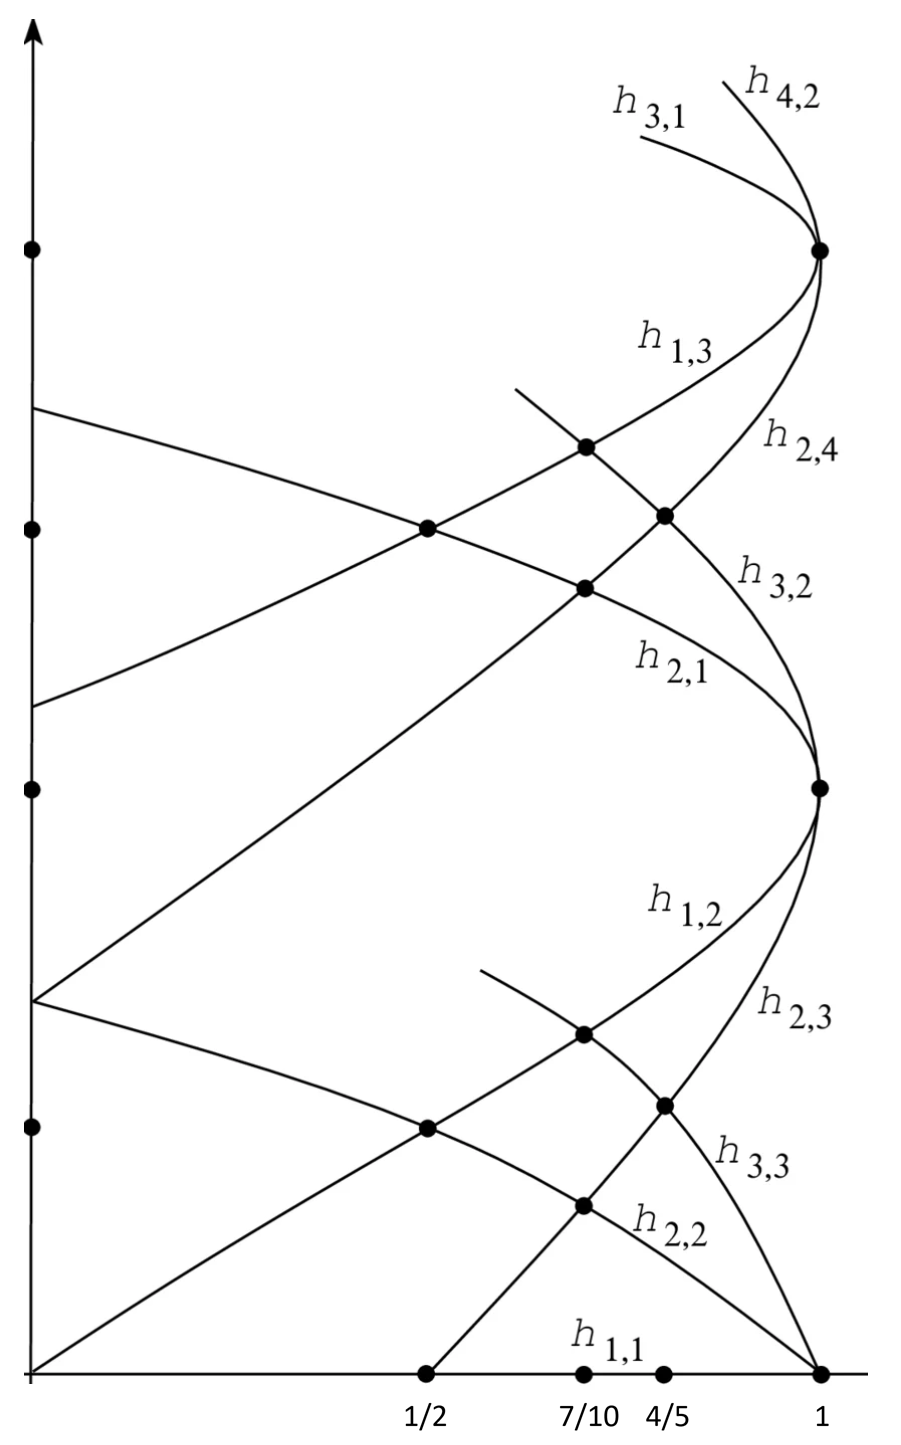
\includegraphics[width=0.9\textwidth]{img/Kac_curves.png}
    \end{minipage}
\end{figure}

\subsubsection{The Physical Role of Null Vectors}

Null vectors are not merely a mathematical curiosity of representation theory; they have profound, direct physical consequences for the dynamics of the conformal field theory.

Because a null state $\ket{\chi}$ is orthogonal to all physical states, it strictly decouples from all physical matrix elements. If a primary field $\Phi(z)$ contains a null state at level $N$ within its conformal family, inserting the corresponding null-state descendant into a correlation function must identically yield zero:
\[
    \langle \chi(z) \Phi_1(z_1) \dots \Phi_n(z_n) \rangle = 0.
\]

Through the state-operator correspondence and the conformal Ward identities, the descendant field $\chi(z)$ can be re-expressed as a specific linear combination of highly complex differential operators acting on the primary field $\Phi(z)$. Therefore, setting the correlation function to zero \uline{translates the existence of the null vector into a strictly homogeneous linear differential equation} that the physical correlation function must satisfy.

In summary, null vectors:
\begin{itemize}
    \item Lead directly to exact differential equations for the conformal blocks.\footnote{We will show this more explicitly in the next chapters.}
    \item Strongly constrain the operator product expansion (OPE) and the fusion rules (the operator algebra).
    \item Are the fundamental mechanism that truncates the spectrum, making rational conformal field theories (like the minimal models) exactly solvable.
\end{itemize}

\subsection{Holomorphic and Full Representations}

Up to this point, our structural analysis has focused entirely on a single chiral sector (the holomorphic Virasoro algebra). However, a physical two-dimensional conformal field theory lives on the complex plane (or a cylinder/torus) and depends on both $z$ and $\bar{z}$.

To construct the full, physical representation space of the theory, we must combine the holomorphic and anti-holomorphic sectors. The complete Hilbert space $\mathcal{H}$ is obtained by taking the direct sum of the tensor products of the physically allowed irreducible representations (where all null submodules have been completely quotiented out):
\[
    \mathcal{H} = \bigoplus_{(h, \bar{h})} N_{h, \bar{h}} \mathcal{L}_{c,h} \otimes \bar{\mathcal{L}}_{c, \bar{h}}.
\]

Here, $\mathcal{L}_{c,h} = \mathcal{V}_{c,h} / \mathcal{N}_{c,h}$ represents the irreducible highest-weight representation of the holomorphic sector, and $\bar{\mathcal{L}}_{c, \bar{h}}$ is its anti-holomorphic counterpart. Each distinct local primary field in the CFT corresponds to one such pair $(h, \bar{h})$, and its full conformal family encompasses the tensor product of the two respective chiral towers.

The non-negative integers $N_{h, \bar{h}}$ are the multiplicities, specifying exactly which primary fields are present in the theory and how many times they appear. These multiplicities cannot be chosen arbitrarily; they are rigidly determined by macroscopic physical consistency requirements, most notably, the requirement of \textbf{modular invariance} of the partition function when the theory is placed on a torus. This elegant factorized structure into chiral and anti-chiral building blocks is the absolute defining hallmark of two-dimensional conformal symmetry.